% Document Type: TeX
\typeout{IF IF IF IF IF IF IF IF IF IF IF IF IF IF IF IF IF IF IF IF IF IF IF}
\newcommand{\ifelse}[2]{#1}
 % Grammatech
% \input{else} % Tech Rep
\documentclass[11pt,twoside,fleqn,openright,titlepage]{cslreport}
%\topmargin 12pt
\topmargin .2in
\textwidth 5.5in
\textheight 7.75in
\oddsidemargin .65in
\evensidemargin .41in
\marginparwidth 0.85in
\marginparsep 0.2in

\raggedbottom
\usepackage{cite,relative,url,alltt,times}
\usepackage{amsfonts,latexsym,amssymb}


%%\usepackage{setspace}%\doublespacing
%
% define variants of the \LaTeX macro that avoid using \sc
% for use in headings
%
\def\BigLaTeX{{\rm L\kern-.36em\raise.3ex\hbox{\smaller\smaller A}\kern-.15em
    T\kern-.1667em\lower.7ex\hbox{E}\kern-.125emX}}
\def\BoldLaTeX{{\bf L\kern-.36em\raise.3ex\hbox{\smaller\smaller\bf A}\kern-.15em
    T\kern-.1667em\lower.7ex\hbox{E}\kern-.125emX}}
\def\BibTeX{{\rm B\kern-.05em{\sc i\kern-.025em b}\kern-.08em
    T\kern-.1667em\lower.7ex\hbox{E}\kern-.125emX}}
%\def\labelitemi{$\bullet$}
\def\labelitemii{$\circ$}
\def\labelitemiii{$\star$}
\def\labelitemiv{$\diamond$}
\newcommand{\boxref}[1]{{\setlength{\fboxsep}{0.5mm}\small\fbox{\ref{#1}}}}
\newcommand{\tcc}{{\sc tcc}}
\newcommand{\tccs}{{\sc tcc}s}
\newcommand{\emacs}{{\sc Emacs}}
\newcommand{\Emacs}{{\sc Emacs}}
\newcommand{\ehdm}{{\sc Ehdm}}
\newcommand{\Ehdm}{{\sc Ehdm}}
\newcommand{\bigEhdm}{E{\smaller HDM}}
\newcommand{\bfehdm}{{\bf E{\smaller\bf HDM}}}
\newcommand{\itehdm}{{\it E{\smaller\it HDM}}}
\newcommand{\slehdm}{{\sl E{\smaller\sl HDM}}}
\newcommand{\murphi}{Mur$\phi$}
\newcommand{\Murphi}{Mur$\phi$}
\newcommand{\tm}{$^{\mbox{\tiny TM}}$}
\newcommand{\hozline}{{\noindent\rule{\textwidth}{0.4mm}}}
\newcommand{\allclear}{\mbox{\boldmath$\stackrel{\raisebox{-.2ex}[0pt][0pt]{$\textstyle\oslash$}}{\displaystyle\bot}$}}
\newenvironment{private}{}{}
\newenvironment{smalltt}{\begin{alltt}\small\tt}{\end{alltt}}
\newenvironment{mysmalltt}{\vspace{-1ex}\begin{alltt}\small\tt}{\end{alltt}\vspace{-1ex}}
\newenvironment{tinyalltt}{\begin{alltt}\tiny\tt}{\end{alltt}}
\newlength{\hsbw}
\newenvironment{slidesession}{\begin{flushleft}
 \setlength{\hsbw}{\linewidth}
 \addtolength{\hsbw}{-\arrayrulewidth}
 \addtolength{\hsbw}{-\tabcolsep}
 \begin{tabular}{@{}|c@{}|@{}}\hline 
 \begin{minipage}[b]{\hsbw}
 \begingroup\mbox{ }\\[-1.6\baselineskip]\begin{alltt}}{\end{alltt}\endgroup\end{minipage}\\ \hline 
 \end{tabular}
 \end{flushleft}}
\newenvironment{dslidesession}{\begin{flushleft}
 \setlength{\hsbw}{\linewidth}
 \addtolength{\hsbw}{-\arrayrulewidth}
 \addtolength{\hsbw}{-\tabcolsep}
 \begin{tabular}{@{}|c@{}|@{}}\hline 
 \begin{minipage}[b]{\hsbw}
 \begingroup\mbox{ }\\[-1.2\baselineskip]\begin{alltt}}{\end{alltt}\endgroup\end{minipage}\\ \hline 
 \end{tabular}
 \end{flushleft}}
\newenvironment{session}{\begin{flushleft}
  \def\baselinestretch{1}
 \setlength{\hsbw}{\linewidth}
 \addtolength{\hsbw}{-\arrayrulewidth}
 \addtolength{\hsbw}{-\tabcolsep}
 \begin{tabular}{@{}|c@{}|@{}}\hline 
 \begin{minipage}[b]{\hsbw}
% \begingroup\small\mbox{ }\\[-1.8\baselineskip]\begin{alltt}}{\end{alltt}\endgroup\end{minipage}\\ \hline
 \begingroup\sessionsize\vspace*{1.2ex}\begin{alltt}}{\end{alltt}\endgroup\end{minipage}\\ \hline
 \end{tabular}
 \end{flushleft}}
\def\extrawidth{0.5in}
\newenvironment{widesession}{\begin{flushleft}
  \def\baselinestretch{1}
 \setlength{\hsbw}{\linewidth}
 \addtolength{\hsbw}{\extrawidth}
 \addtolength{\hsbw}{-\arrayrulewidth}
 \addtolength{\hsbw}{-\tabcolsep}
 \begin{tabular}{@{}|c@{}|@{}}\hline 
 \begin{minipage}[b]{\hsbw}
% \begingroup\small\mbox{ }\\[-1.8\baselineskip]\begin{alltt}}{\end{alltt}\endgroup\end{minipage}\\ \hline
 \begingroup\sessionsize\vspace*{1.2ex}\begin{alltt}}{\end{alltt}\endgroup\end{minipage}\\ \hline
 \end{tabular}
 \end{flushleft}}
\def\invisiblespec{\comment}
\def\endinvisiblespec{\endcomment}
\newenvironment{sessionlab}[1]{\begin{flushleft}
 \setlength{\hsbw}{\linewidth}
 \addtolength{\hsbw}{-\arrayrulewidth}
 \addtolength{\hsbw}{-\tabcolsep}
 \begin{tabular}{@{}|c@{}|@{}}\hline 
 \begin{minipage}[b]{\hsbw}
 \vspace*{-.5pt}
 \begin{flushright}
 \rule{0.01in}{.15in}\rule{0.9in}{0.01in}\hspace{-0.95in}
 \raisebox{0.04in}{\makebox[0.9in][c]{\footnotesize #1}}
 \end{flushright}
 \vspace*{-.57in}
 \begingroup\small\vspace*{1.0ex}\begin{alltt}}{\end{alltt}\endgroup\end{minipage}\\ \hline 
 \end{tabular}
 \end{flushleft}}
\newcounter{sessioncount}
\setcounter{sessioncount}{0}
% ---------------------------------------------------------------------
% Macros for little PVS sessions displayed in boxes.
%
% Usage: (1) \setcounter{sessioncount}{1} resets the session counter
%
%	 (2) \begin{session*}\label{thissession}
%	      .
%	       < lines from PVS session >
%	      .
%	     \end{session*}
%
%            typesets the session in a numbered box in ALLTT mode.
%
%  session instead of session* produces unnumbered boxes
%
% ---------------------------------------------------------------------
\newenvironment{session*}{\begin{flushleft}
 \refstepcounter{sessioncount}
 \setlength{\hsbw}{\linewidth}
 \addtolength{\hsbw}{-\arrayrulewidth}
 \addtolength{\hsbw}{-\tabcolsep}
 \begin{tabular}{@{}|c@{}|@{}}\hline 
 \begin{minipage}[b]{\hsbw}
 \vspace*{-.5pt}
 \begin{flushright}
 \rule{0.01in}{.15in}\rule{0.3in}{0.01in}\hspace{-0.35in}
 \raisebox{0.04in}{\makebox[0.3in][c]{\footnotesize \thesessioncount}}
 \end{flushright}
 \vspace*{-.57in}
 \begingroup\small\vspace*{1.0ex}\begin{alltt}}{\end{alltt}\endgroup\end{minipage}\\ \hline 
 \end{tabular}
 \end{flushleft}}
\def\sessionsize{\small}
\def\smallsessionsize{\small}
\newenvironment{smallsession}{\begin{flushleft}
 \setlength{\hsbw}{\linewidth}
 \addtolength{\hsbw}{-\arrayrulewidth}
 \addtolength{\hsbw}{-\tabcolsep}
 \begin{tabular}{@{}|c@{}|@{}}\hline 
 \begin{minipage}[b]{\hsbw}
 \begingroup\smallsessionsize\mbox{ }\\[-1.8\baselineskip]\begin{alltt}}{\end{alltt}\endgroup\end{minipage}\\ \hline 
 \end{tabular}
 \end{flushleft}}
\newenvironment{spec}{\begin{flushleft}
 \setlength{\hsbw}{\textwidth}
 \addtolength{\hsbw}{-\arrayrulewidth}
 \addtolength{\hsbw}{-\tabcolsep}
 \begin{tabular}{@{}|c@{}|@{}}\hline 
 \begin{minipage}[b]{\hsbw}
 \begingroup\small\mbox{
}\\[-0.2\baselineskip]}{\endgroup\end{minipage}\\ \hline 
 \end{tabular}
 \end{flushleft}}
\newcommand{\memo}[1]{\mbox{}\par\vspace{0.25in}%
\setlength{\hsbw}{\linewidth}%
\addtolength{\hsbw}{-2\fboxsep}%
\addtolength{\hsbw}{-2\fboxrule}%
\noindent\fbox{\parbox{\hsbw}{{\bf Memo: }#1}}\vspace{0.25in}}
\newcommand{\nb}[1]{\mbox{}\par\vspace{0.25in}\setlength{\hsbw}{\linewidth}\addtolength{\hsbw}{-1.5ex}\noindent\fbox{\parbox{\hsbw}{{\bf Note: }#1}}\vspace{0.25in}}
%\newcommand{\comment}[1]{}
%\def\comment#1{}   % Shankar doesn't like this, but the other defn
%		   % gives me errors
\newcommand{\exfootnote}[1]{}
%\newcommand{\ifelse}[2]{#1}
\sloppy
\clubpenalty=100000
\widowpenalty=100000
%\displaywidowpenalty=100000
\setcounter{secnumdepth}{3} 
\setcounter{tocdepth}{3}
\setcounter{topnumber}{9}
\setcounter{bottomnumber}{9}
\setcounter{totalnumber}{9}
\renewcommand{\topfraction}{.99}
\renewcommand{\bottomfraction}{.99}
\renewcommand{\floatpagefraction}{.01}
\renewcommand{\textfraction}{.2}
\font\largett=cmtt10 scaled\magstep1
\font\Largett=cmtt10 scaled\magstep2
\font\hugett=cmtt10 scaled\magstep3
\newcommand{\take}[1]{\\\hozline\paragraph*{From file {\tt #1}}\input{#1}\hozline}
\newlength{\sblen}
\newlength{\overhang}
%\setlength{\overhang}{0pt}
\newenvironment{sidebar}%
{\begin{figure}[htb]%
 \begin{Sbox}%
 \setlength{\sblen}{\textwidth}%
 \addtolength{\sblen}{-2\fboxsep}%
 \addtolength{\sblen}{-2\fboxrule}%
 \addtolength{\sblen}{-\overhang}%
 \begin{minipage}{\sblen}}%
{\end{minipage}\end{Sbox}\shadowbox{\TheSbox}\end{figure}}
\newenvironment{sidepage}%
{\begin{figure}[p]%
 \begin{Sbox}%
 \setlength{\sblen}{\textwidth}%
 \addtolength{\sblen}{-2\fboxsep}%
 \addtolength{\sblen}{-2\fboxrule}%
 \addtolength{\sblen}{-\overhang}%
 \begin{minipage}{\sblen}\parindent=1.5em}%
{\end{minipage}\end{Sbox}\shadowbox{\TheSbox}\end{figure}}
\def\SetFigFont#1#2#3{\rm}
\newcommand{\ul}[1]{\underline{\rule[-0.50ex]{0pt}{1ex}#1}}
\newcommand{\ttilde}{\raisebox{-.5ex}{\tt \~{}}}
\newcommand{\excite}[1]{}
%\newcommand{\hand}{$\Rightarrow$}
\newcommand{\hand}{\ ($\Rightarrow$)}
\newcommand{\nls}{\\\hspace*{1em}}
\def\srilogo{
\includegraphics[height=18mm]{srilogo}}
\newtheorem{definition}{Definition}
\newtheorem{lemma}{Lemma}
\newtheorem{theorem}{Theorem}

%\input{mathprel}
\pagenumbering{roman} 
\setcounter{page}{0} 
%\input{nomemos}
\makeatletter
\@ifundefined{pdfoutput}%
{\usepackage[bookmarks=true,hyperindex=true]{hyperref}}%
{%\usepackage[pdftex,dvipsnames,usenames]{color}%
\usepackage[chapter]{tocbibind}%
\usepackage[bookmarks=true,hyperindex=true,colorlinks=true,linkcolor=blue,citecolor=blue,backref=page,pagebackref=true,plainpages=false,pdfpagelabels]{hyperref}%
}%
\makeatother

%% \renewcommand{\baselinestretch}{1.5}

\begin{document}
\ifelse{\cslreportnumber{}}{}
\begin{titlepage}
\date{\today}
\author{Bruno Dutertre\\
Computer Science Laboratory\\
SRI International\\
Menlo Park CA 94025 USA
}
\title{\bf Yices~2 Manual}
\end{titlepage}

\maketitle
\cleardoublepageblank
\tableofcontents
%\listoffigures
\cleardoublepage
\setcounter{page}{0}
\pagenumbering{arabic}


\chapter{Introduction}

This manual is an introduction to the logic, language, and
architecture of the Yices~2 SMT solver. Yices is developed in SRI
International's Computer Science Laboratory and is distributed
free-of-charge for personal use, under the terms of the Yices
License~\ref{license}.  To discuss alternative license terms, please
contact us at \texttt{fm-license@csl.sri.com}.

Yices can be downloaded at \url{http://yices.csl.sri.com}. The Yices
website provides the latest release and information about Yices.
For bug reports and questions about Yices, please contact us via
the Yices mailing lists:
\begin{itemize}
\item To report a bug, send e-mail to \texttt{yices-bugs@csl.sri.com}.

  Please include enough information in your bug report to enable us
  to reproduce the problem.

\item If you have any questions about Yices usage or installation, 
   send e-mail to \texttt{yices-help@csl.sri.com}.
\end{itemize}



\chapter{Yices~2 Language}
\label{language}

Yices~2 specifications are written in a typed logic. The language is
intended to be simple enough for efficient processing by the tool and
expressive enough for most applications. The Yices~2 language is
similar to the logic supported by Yices~1, but the most complex type
constructs have been removed.


\section{Type System}

Yices~2 has a few built-in types for primitive objects:
\begin{itemize}
\item The arithmetic types \texttt{int} and \texttt{real}
\item The Boolean type \texttt{bool}
\item The type \texttt{(bitvector k)} of bitvectors of size $k$,
 where $k$ is a positive integer.
\end{itemize}
All these built-in types are {\em atomic\/}. The set of atomic types
can be extended by declaring new {\em uninterpreted types\/} and {\em
  scalar types\/}. An uninterpreted type denotes a nonempty
collection of objects with no cardinality constraint. A scalar type
denotes a nonempty, {\em finite\/} set of objects. The cardinality of
a scalar type is defined when the type is created.

\medskip

In addition to the atomic types, Yices~2 provides constructors for
tuple and function types. The set of all Yices~2 types can be defined
inductively as follows:
\begin{itemize}
\item Any atomic type $\tau$ is a type.
\item If $n>0$ and $\sigma_1,\ldots,\sigma_n$ are $n$ types, then
  $\sigma = (\sigma_1 \times \ldots \times \sigma_n)$ is a type. Objects
  of type $\sigma$ are tuples $(x_1,\ldots, x_n)$ where $x_i$ is an
  object of type $\sigma_i$.
\item If $n>0$ and $\sigma_1,\ldots,\sigma_n$ and $\tau$ are types,
  then $\sigma = (\sigma_1\times \ldots\times\sigma_n \rightarrow
  \tau)$ is a type. Objects of type $\sigma$ are functions of domain
  $\sigma_1\times\ldots\times\sigma_n$ and range $\tau$.
\end{itemize}
By construction, all the types are nonempty. Yices does not have a
specific type constructor for arrays since the logic does not
distinguish between arrays and functions. For example, an array
indexed by integers is simply a function of domain $\mathtt{int}$.

\medskip

Yices~2 uses a simple form of subtyping. Given two types $\sigma$ and
$\tau$, let $\sigma\sqsubset\tau$ denote that $\sigma$ is a subtype of
$\tau$. Then the subtype relation is defined by the following rules:
\begin{itemize}
\item $\tau\sqsubset\tau$ (any type is a subtype of itself)
\item $\mathtt{int}\sqsubset\mathtt{real}$ (the integers form a subtype of the reals)
\item If $\sigma_1\sqsubset\tau_1,\ldots,\sigma_n\sqsubset\tau_n$ then
$(\sigma_1\times \ldots\times\sigma_n)\sqsubset (\tau_1\times\ldots\times\tau_n)$.
\item If $\tau\sqsubset\tau'$ then
  $(\sigma_1\times\ldots\times\sigma_n\rightarrow\tau)\sqsubset
  (\sigma_1\times\ldots\times\sigma_n\rightarrow\tau')$. 
\end{itemize}
For example, the type $(\mathtt{int}\times\mathtt{int})$ (pairs of
integers) is a subtype of $(\mathtt{real}\times\mathtt{real})$ (pairs of reals).

Two types, $\tau$ and $\tau'$, are said to be {\em compatible\/} if
they have a common supertype, that is, if there exists a type $\sigma$
such that $\tau\sqsubset\sigma$ and $\tau'\sqsubset\sigma$.  If that
is the case, then there exists a unique minimal supertype among all
the common supertypes. We denote the minimal supertype of $\tau$ and
$\tau'$ by $\tau\sqcup\tau'$. By definition, we then have
$$\tau\sqsubset\sigma~~\mathtt{and}~~\tau'\sqsubset\sigma~~\Rightarrow~~\tau\sqcup\tau'\:\sqsubset\:\sigma.$$
For example, the tuple types
$\tau=(\mathtt{int}\times\mathtt{real}\times\mathtt{int})$ and
$\tau=(\mathtt{int}\times\mathtt{int}\times\mathtt{real})$ are
compatible. Their minimal supertype is $\tau\sqcup\tau' =
(\mathtt{int}\times\mathtt{real}\times\mathtt{real})$. The type
$(\mathtt{real}\times\mathtt{real}\times\mathtt{real})$ is also a
common supertype of $\tau$ and $\tau'$ but it is not minimal.


\section{Terms and Formulas}

In Yices~2, the atomic terms include the Boolean constants
(\texttt{true} and \texttt{false}) as well as arithmetic and bitvector
constants. 

When a scalar type $\tau$ of cardinality $n$ is declared, $n$ distinct
constant $c_1,\ldots,c_n$ of type $\tau$ are also implicitly
defined. In the Yices~2 syntax, this is done via a declaration of the
form:
\begin{small}
\begin{verbatim}
  (define-type tau (scalar c1 ... cn))
\end{verbatim}
\end{small}
An equivalent functionality is provided by the Yices API. The API
allows one to create a new scalar type and to access $n$ constants of
that type indexed by integers between $0$ and $n-1$ (check
file \texttt{include/yices.h} for explanations).

The user can also declare {\em uninterpreted constants\/} of arbitrary
types. Informally, uninterpreted constants of type $\tau$ can be
considered like global variables, but Yices (in particular the Yices
API) makes a distinction between {\em variables\/} of type $\tau$ and
{\em uninterpreted constants\/} of type $\tau$. In the Yices API,
variables are used to build quantified expressions and to support term
substitutions. Free variables are not allowed to occur in assertions.

\medskip

The term constructors include the common Boolean operators
(conjunction, disjunction, negation, implication, etc.), an
if-then-else constructor, equality, function application, and tuple
constructor and projection. In addition, Yices provides
an \texttt{update} operator that can be applied to arbitrary
functions. The type-checking rules for these primitive operators are
described in Figure~\ref{type-checking}, where the notation $t::\tau$
means ``term $t$ has type $\tau$''.

There are no separate syntax or constructors for formulas. In Yices~2,
a formula is simply a term of Boolean type.

\begin{figure}
\begin{center}
Boolean Operators\\[1ex]
\begin{displaymath}
\hspace{3em}
\frac{~~t::\mathtt{bool}~~}{~~(\mathtt{not}\ t)::\mathtt{bool}~~}
\hspace{2em}
\frac{~~t_1::\mathtt{bool}~~~t_2::\mathtt{bool}~~}{~~(\mathtt{implies}\ t_1\ t_2)::\mathtt{bool}~~}
\end{displaymath}
\begin{displaymath}
\hspace{2em}
\frac{~~t_1::\mathtt{bool}\ldots t_n::\mathtt{bool}~~}{~~(\mathtt{or}\ t_1\ldots t_n)::\mathtt{bool}~~}
\hspace{2em}
\frac{~~t_1::\mathtt{bool}\ldots t_n::\mathtt{bool}~~}{~~(\mathtt{and}\ t_1\ldots t_n)::\mathtt{bool}~~}
\end{displaymath}
\vspace*{2ex}
Equality\\[1ex]
\begin{displaymath}
\hspace{2em}
\frac{~~t_1::\tau_1~~~t_2::\tau_2~~}{~~(t_1 = t_2)::\mathtt{bool}~~}\mbox{~~provided $\tau_1$ and $\tau_2$ are compatible}
\end{displaymath}
\vspace*{2ex}
If-then-else\\[1ex]
\begin{displaymath}
\hspace{2em}
\frac{~~c::\mathtt{bool}~~~t_1::\tau_1~~~t_2::\tau_2~~}{~~(\mathtt{ite}\ c\ t_1\ t_2)::\tau_1\sqcup\tau_2~~}
\mbox{~~provided $\tau_1$ and $\tau_2$ are compatible}
\end{displaymath}
\vspace*{2ex}
Tuple Constructor and Projection\\[1ex]
\begin{displaymath}
\hspace{2em}
\frac{~~t_1::\tau_1 \ldots t_n::\tau_n~~}{~~(\mathtt{tuple}\ t_1\ldots t_n)::(\tau_1\times\ldots\times\tau_n)~~}
\hspace{2em}
\frac{~~t::(\tau_1\times\ldots\times\tau_n)~~}{~~(\mathtt{select}_i\ t)::\tau_i~~}
\end{displaymath}
\vspace*{2ex}
Function Application\\[1ex]
\begin{displaymath}
\hspace{2em}
\frac{~~f::(\tau_1\times\ldots\times\tau_n\rightarrow\tau)~~~t_1::\sigma_1\ldots t_n::\sigma_n~~~\sigma_1\sqsubset\tau_1\ldots\sigma_n\sqsubset\tau_n~~}{~~~(f\ t_1\ldots t_n)::\tau~~~}
\end{displaymath}
\vspace*{2ex}
Function Update\\[1ex]
\begin{displaymath}
\hspace{2em}
\frac{~~f::(\tau_1\times\ldots\times\tau_n\rightarrow\tau)~~~t_1::\sigma_1\ldots t_n::\sigma_n~~v::\sigma~~\sigma_i\sqsubset\tau_i~~~\sigma\sqsubset\tau~~}{~~~(\mathtt{update}\ f\ t_1\ldots t_n\ v)::(\tau_1\times\ldots\times\tau_n\rightarrow\tau)~~~}
\end{displaymath}
\vspace*{2ex}
\end{center}
\caption{Primitive Operators and Type Checking}
\label{type-checking}
\end{figure}

The semantics of most of these operators is standard. The update
operator for functions is characterized by the following
axioms\footnote{These are the main axioms of the McCarthy theory of arrays.}:
\begin{eqnarray*}
((\mathtt{update}\ f\ t_1\ldots t_n\ v)\ t_1\ldots t_n) & = & v \\
u_1\neq t_1\vee\ldots\vee u_n\neq t_n\Rightarrow((\mathtt{update}\ f\ t_1\ldots t_n\ v)\ u_1\ldots u_n) & = & (f\ u_1\ldots u_n)
\end{eqnarray*}
In other words, $(\mathtt{update}\ f\ t_1\ldots t_n\ v)$ is the
function equal to $f$ at all points except $(t_1,\ldots,t_n)$.
Informally, if $f$ is interpreted as an array then the update
corresponds to ``storing'' $v$ at position $t_1,\ldots,t_n$ in the
array.  Reading the content of the array is nothing other than function
application: $(f\ i_1\ldots i_n)$ is the content of the array at
position $i_1,\ldots, i_n$.

\bigskip

The full Yices~2 language has a few more operators not described here,
and it includes existential and universal quantifiers. We do not
describe the type-checking rules for quantifiers here since Yices~2
does not have a solver for quantified formulas at this point.


\section{Supported Theories}

In addition to the generic operators presented previously, the Yices
language includes the standard arithmetic operators and a rich set of
bitvector operators.

\subsection{Arithmetic}

Arithmetic constants are arbitrary precision integers and rationals.
Although Yices uses exact arithmetic, rational constants can be
written using standard floating-point notation. Internally, Yices
converts floating-point input to rationals. For example, the
floating-point expression $3.04e-1$ is converted to $304/1000$. 

The Yices language supports the traditional arithmetic
operators (i.e., addition, subtraction, multiplication) with the
exception that it does not allow division by a non constant, to avoid
issues related to division by zero. For example, the expression $(x +
4y)/3$ is allowed, but $3/(x + 4y)$ is not. The arithmetic predicates
are the usual comparison operators, including both strict and
nonstrict inequalities.

The language allows nonlinear polynomials but this is not fully
supported by the tool at this time. Yices~2 can solve problems
involving real and integer linear arithmetic, but it does not yet
include a solver for nonlinear arithmetic.


\subsection{Bitvectors}

Yices supports all the bitvector operators defined in the SMT-LIB
standard~\cite{SMTLIB12:2006}. The most commonly used operators are
listed in Table~\ref{bitvectors}. They include bitvector arithmetic
(where bitvectors are interpreted either as unsigned integers or as
signed integers in two's complement representation), logical operators
such as bitwise OR or AND, logical and arithmetic shifts,
concatenation, and extraction of subvectors. Other operators are
defined in the theory QF\_BV of SMT-LIB
(cf.~\url{http://combination.cs.uiowa.edu/smtlib}); all of them are
supported by Yices~2.

\begin{table}
%% \renewcommand{\arraystretch}{1}
\begin{tabular}{|l|l|}
\hline 
Operator and Type & Meaning\\
\hline
$\mathtt{bvadd}::((\mathtt{bv}\ n)\times (\mathtt{bv}\ n) \rightarrow (\mathtt{bv}\ n))$ &
addition\\
$\mathtt{bvsub}::((\mathtt{bv}\ n)\times (\mathtt{bv}\ n) \rightarrow (\mathtt{bv}\ n))$ &
subtraction\\
$\mathtt{bvmul}::((\mathtt{bv}\ n)\times (\mathtt{bv}\ n) \rightarrow (\mathtt{bv}\ n))$ &
multiplication\\
$\mathtt{bvneg}::\mathtt{bv}\ n) \rightarrow (\mathtt{bv}\ n))$ &
2's complement opposite\\
\hline
$\mathtt{bvudiv}::((\mathtt{bv}\ n)\times (\mathtt{bv}\ n) \rightarrow (\mathtt{bv}\ n))$ &
quotient in unsigned division \\
$\mathtt{bvudiv}::((\mathtt{bv}\ n)\times (\mathtt{bv}\ n) \rightarrow (\mathtt{bv}\ n))$ &
remainder in unsigned division \\
$\mathtt{bvsdiv}::((\mathtt{bv}\ n)\times (\mathtt{bv}\ n) \rightarrow (\mathtt{bv}\ n))$ &
quotient in signed division \\
& with rounding toward zero\\
$\mathtt{bvsrem}::((\mathtt{bv}\ n)\times (\mathtt{bv}\ n) \rightarrow (\mathtt{bv}\ n))$ &
remainder in signed division \\
& with rounding toward zero\\
$\mathtt{bvsmod}::((\mathtt{bv}\ n)\times (\mathtt{bv}\ n) \rightarrow (\mathtt{bv}\ n))$ &
remainder in signed division\\
& with rounding toward $-\infty$\\
\hline 
$\mathtt{bvule}::((\mathtt{bv}\ n)\times (\mathtt{bv}\ n) \rightarrow \mathtt{bool}$ &
unsigned less than or equal\\
$\mathtt{bvuge}::((\mathtt{bv}\ n)\times (\mathtt{bv}\ n) \rightarrow \mathtt{bool}$ &
unsigned greater than or equal\\
$\mathtt{bvult}::((\mathtt{bv}\ n)\times (\mathtt{bv}\ n) \rightarrow \mathtt{bool}$ &
unsigned less than\\
$\mathtt{bvugt}::((\mathtt{bv}\ n)\times (\mathtt{bv}\ n) \rightarrow \mathtt{bool}$ &
unsigned greater than\\
$\mathtt{bvsle}::((\mathtt{bv}\ n)\times (\mathtt{bv}\ n) \rightarrow \mathtt{bool}$ &
unsigned less than or equal\\
$\mathtt{bvsge}::((\mathtt{bv}\ n)\times (\mathtt{bv}\ n) \rightarrow \mathtt{bool}$ &
unsigned greater than or equal\\
$\mathtt{bvslt}::((\mathtt{bv}\ n)\times (\mathtt{bv}\ n) \rightarrow \mathtt{bool}$ &
unsigned less than\\
$\mathtt{bvsgt}::((\mathtt{bv}\ n)\times (\mathtt{bv}\ n) \rightarrow \mathtt{bool}$ &
unsigned greater than\\
\hline
$\mathtt{bvand}::((\mathtt{bv}\ n)\times (\mathtt{bv}\ n) \rightarrow (\mathtt{bv}\ n))$ &
bitwise and\\
$\mathtt{bvor}::((\mathtt{bv}\ n)\times (\mathtt{bv}\ n) \rightarrow (\mathtt{bv}\ n))$ &
bitwise or\\
$\mathtt{bvnot}::((\mathtt{bv}\ n) \rightarrow (\mathtt{bv}\ n))$ &
bitwise negation\\
$\mathtt{bvxor}::((\mathtt{bv}\ n)\times (\mathtt{bv}\ n) \rightarrow (\mathtt{bv}\ n))$ &
bitwise exclusive or\\
\hline
$\mathtt{bvshl}::((\mathtt{bv}\ n)\times (\mathtt{bv}\ n) \rightarrow (\mathtt{bv}\ n))$ &
shift left\\
$\mathtt{bvlshr}::((\mathtt{bv}\ n)\times (\mathtt{bv}\ n) \rightarrow (\mathtt{bv}\ n))$ &
logical shift right\\
$\mathtt{bvashr}::((\mathtt{bv}\ n)\times (\mathtt{bv}\ n) \rightarrow (\mathtt{bv}\ n))$ &
arithmetic shift right\\
\hline
$\mathtt{bvconcat}::((\mathtt{bv}\ n)\times (\mathtt{bv}\ m) \rightarrow (\mathtt{bv}\ n+m))$ &
concatenation \\
$\mathtt{bvextract}_{i,j}$$((\mathtt{bv}\ n) \rightarrow (\mathtt{bv}\ m))$ &
extract bits $i$ down to $j$ \\
& form a bitvector of size $n$ \\
\hline
\end{tabular}
\caption{Bitvector Operators}
\label{bitvectors}
\end{table}


The semantics of all the bitvector operators is defined in the SMT-LIB~1.2
standard.  Yices~2 follows the standard except for the case of
division by zero.  In SMT-LIB, the result of a division by zero is
an unspecified value, but one must ensure that the division operators are
functional. In other words, SMT-LIB does not specify the result of
$(\mathtt{bvudiv}\ a\ b)$ if $b$ is the zero vector, but
$(\mathtt{bvudiv}\ a\ b)$ and $(\mathtt{bvudiv}\ c\ b)$ must be equal
whenever $a = c$, even if $b$ is the zero vector. Yices~2 uses a
simpler semantics (inspired from the BTOR
format~\cite{Brummayer-etal:2008}): 
\begin{itemize}
\item {\bf Unsigned Division:} If $b$ is the zero bitvector of $n$ bits then 
\begin{eqnarray*}
(\mathtt{bvudiv}\ a\ b) & = & \mathtt{0b111...1} \\
(\mathtt{bvurem}\ a\ b) & = & a
\end{eqnarray*}
In general, the quotient $(\mathtt{bvudiv}\ a\ b)$ is the largest
unsigned integer that can be represented on $n$ bits, and is smaller than $a/b$, 
and the following identity holds for all bitvectors $a$ and $b$
\begin{eqnarray*}
a & = & (\mathtt{bvadd}\ (\mathtt{bvmul}\ (\mathtt{bvudiv}\ a\ b)\ b)\ (\mathtt{bvurem}\ a\ b)).
\end{eqnarray*}

\item {\bf Signed Division:} If $b$ is the zero bitvector of $n$ bits then 
\begin{eqnarray*}
(\mathtt{bvsdiv}\ a\ b) & = & \mathtt{0b000..01}~~\mbox{\rm if $a$ is negative} \\
(\mathtt{bvsdiv}\ a\ b) & = & \mathtt{0b111...1}~~\mbox{\rm if $a$ is non-negative} \\
(\mathtt{bvsrem}\ a\ b) & = & a \\
(\mathtt{bvsmod}\ a\ b) & = & a
\end{eqnarray*}
\end{itemize}




\chapter{Yices~2 Architecture}
\label{architecture-chapter}

Yices~2 relies on a simpler language and type system than Yices~1. We
have also completely redesigned the architecture to make Yices~2
easier to maintain and develop. The new architecture supports new
features, such as the possibility to maintain several contexts in
parallel.

\section{Main Components}

The Yices~2 software can be conceptually decomposed into three main
modules:
\begin{description}
\item[Term Database] Yices~2 maintains a global database in which all
  terms and types are stored. Yices~2 provides an API for constructing terms,
  formulas, and types in this database.

\item[Context Management] A context is a central data structure that
  stores asserted formulas. Each context contains a set of assertions
  to be checked for satisfiability. The context-management API supports
  operations for creating and initializing contexts, for asserting
  formulas into a context, and for checking the satisfiability of the
  asserted formulas. Several contexts can be constructed and
  manipulated independently. 

  Contexts are highly customizable. Each context can be configured to
  support a specific theory, and to use a specific solver or
  combination of solvers.

\item[Model Management] If the set of formulas asserted in a context
  is satisfiable, then one can construct a model of the formulas. The
  model maps symbols of the formulas to concrete values (e.g., integer
  or rational values or bitvector constants). The API provides
  functions to build and query models.
\end{description}

Figure~\ref{top-level-architecture} shows the top-level architecture
of Yices~2, divided into the three main modules. Each context consists
of two separate components: The {\em solver\/} employs a Boolean
satisfiability solver and decision procedures for determining whether
the formulas asserted in the context are satisfiable.  The
\emph{internalizer\/} converts the format used by the term database
into the internal format used by the solver. In particular, the
internalizer rewrites all formulas in conjunctive normal form, which is
used by the internal SAT solver.
\begin{figure}
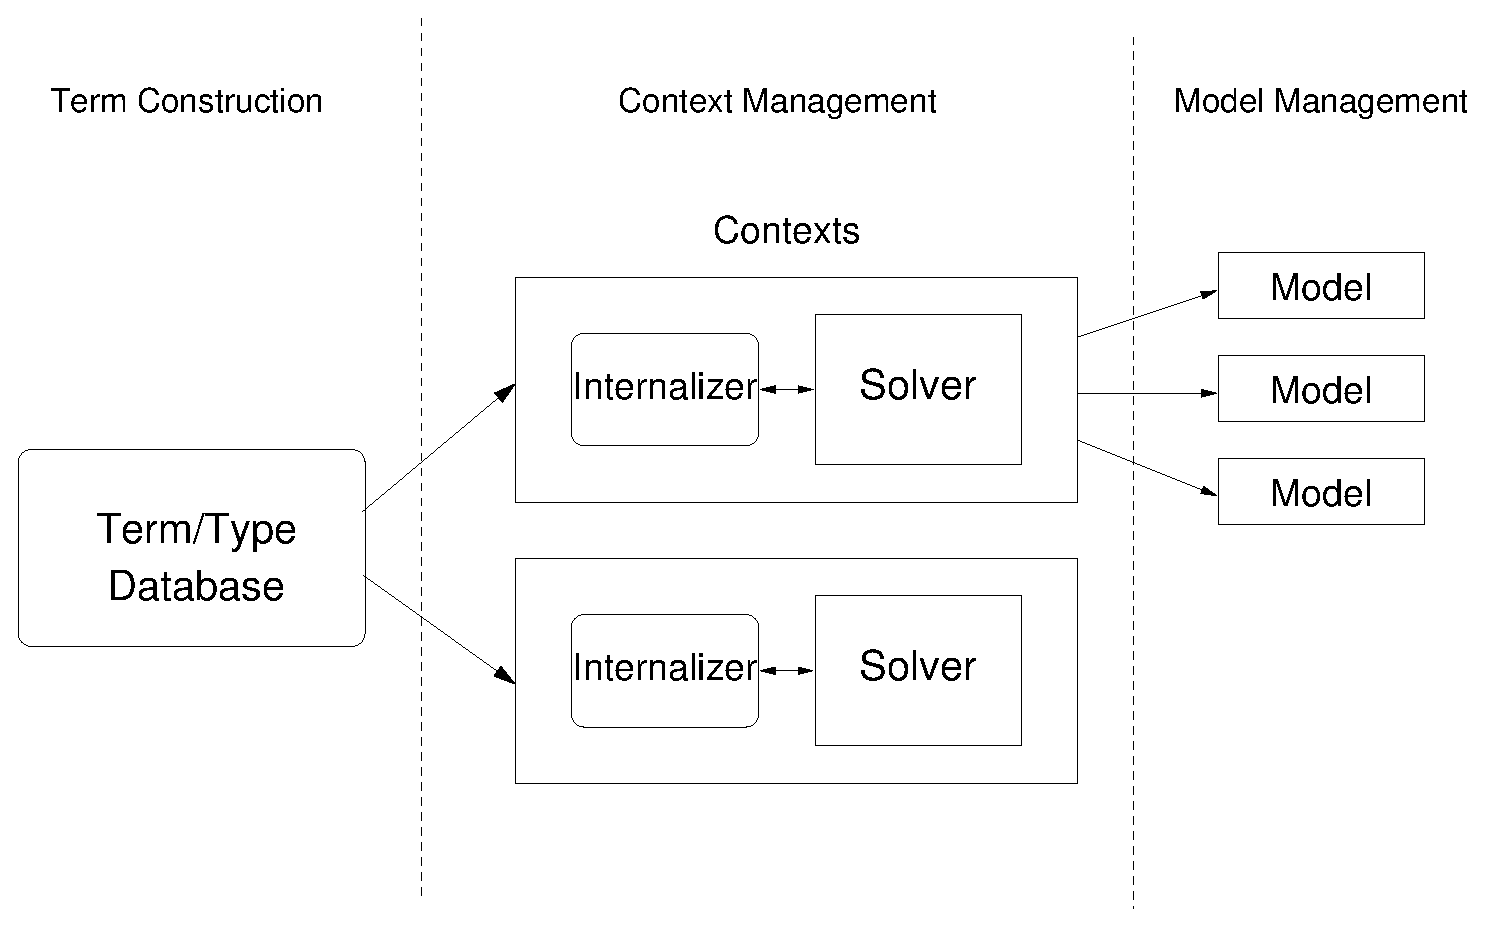
\includegraphics[width=14cm]{yices2-toplevel}
\caption{Top-level Yices~2 Architecture}
\label{top-level-architecture}
\end{figure}


\section{Solvers}

In Yices~2, it is possible to select a different solver (or combination
of solvers) for the problem of interest. Each context can thus be
configured for a specific class of formulas. For example, one can use
a solver specialized for linear arithmetic, or use a solver that
supports the full Yices~2 language. Figure~\ref{solver-architecture}
shows how the most general solver is built. A major component of all
solvers is a SAT solver based on the Davis-Putnam-Logemann-Loveland
(DPLL) procedure. The SAT solver is coupled with one or more so-called
\emph{theory solvers}. Each theory solver implements a decision
procedure for a particular theory. Currently, Yices~2 includes four
main theory solvers:
\begin{itemize}
\item The \emph{UF Solver} deals with the theory of uninterpreted
  functions with equality\footnote{UF stands for uninterpreted
    functions.}. It implements a decision procedure based on computing
  congruence closures, similar to the Simplify
  system~\cite{Detlefs-etal:JACM2005}.
\item The \emph{Arithmetic Solver} deals with linear integer and real
  arithmetic.  It implements a decision procedure based on the Simplex
  algorithm~\cite{DutertredeMoura:cav06,DutertredeMoura:report06}.
\item The \emph{Bitvector Solver} deals with the theory of bitvectors.
\item The \emph{Array Solver} implements a decision procedure for
  McCarthy's theory of arrays.
\end{itemize}


\begin{figure}
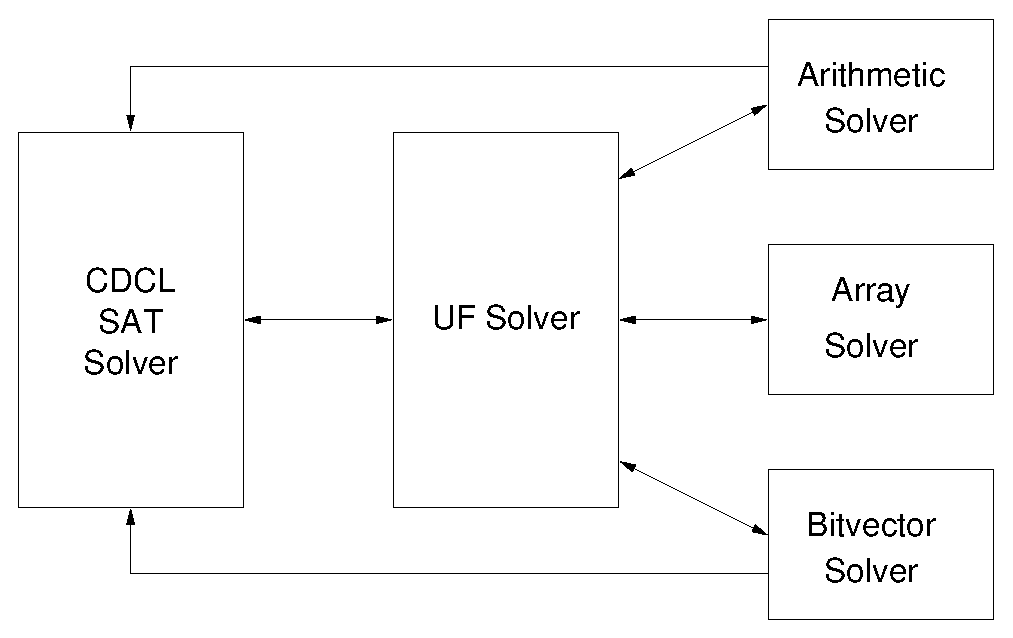
\includegraphics[width=12cm]{yices2-architecture}
\caption{Solver Components}
\label{solver-architecture}
\end{figure}


Yices~2 employs a modular solver architecture. It is possible to
remove some of the components of Figure~\ref{solver-architecture} to
build simpler and more efficient solvers that are specialized for
specific classes of formulas. For example, a solver for pure
arithmetic can be built by directly attaching the arithmetic solver
to the DPLL SAT solver. Similarly, Yices~2 can be specialized for pure
bitvector problems, or for problems combining uninterpreted functions,
arrays, and bitvectors (by removing the arithmetic solver).

Yices~2 combines several theory solver using the Nelson-Oppen
method~\cite{NelsonOppen79}.  The UF solver is essential for this
purpose; it coordinates the different theory solvers and ensures
global consistency. The other solvers (for arithmetic, arrays, and
bitvectors) communicate only with the central UF solver and never
directly with each other. This property considerably simplifies the
design and implementation of theory solvers.


\chapter{\texttt{yices}}
\label{yices-shell}

The Yices~2 distribution includes a tool for processing input written
in the Yices~2 language. This tool is callled \texttt{yices}
(or \texttt{yices.exe} in the Windows and Cygwin distributions).  The
syntax and the set of commands supported by \texttt{yices} are
explained in the file \texttt{doc/YICES-LANGUAGE} included in the
distribution. Several example specifications are also included in
the \texttt{examples/} directory.

By default, the \texttt{yices} tool supports the combination of
arithmetic, uninterpreted functions and arrays. It builds a context
that includes the Simplex, UF, and Array solvers. This can be changed 
by giving command-line arguments to the tool. Try \texttt{yices --help} for
more details.


\chapter{\texttt{yices-smt}}
\label{yices-smt}

Another tool included in the distribution can process input written in
the SMT-LIB notation. This tool is called \texttt{yices-smt}
(or \texttt{yices-smt.exe}). It is included in the \texttt{bin}
directory.  Currently, this tool supports version~1.2 of
SMT-LIB. Support for the more recent SMT-LIB~2 will be provided in
future releases.


\chapter{Yices API}
\label{yices-api}

The distribution includes a library and header files for embedding
Yices in other software. The main header file is \texttt{yices.h}
which includes all the API. The API functions are documented in this
header file. More complete and detailed documentation on the Yices~2
API will be provided at the Yices
website \url{http://yices.csl.sri.com/}.


\chapter{Yices License Terms}
\label{license}

Before downloading and using Yices, you will be asked to agree to the
Yices license terms reproduced below. SRI is open to distributing
Yices under other agreements. Contact us
at \texttt{fm-licencing@csl.sri.com} to discuss alternative licence
terms.

\begin{footnotesize}
\begin{verbatim}
END-USER LICENSE AGREEMENT

IMPORTANT - READ CAREFULLY.  Be  sure to carefully read and understand
all of the rights and  restrictions described in this End-User License
Agreement ("EULA").  You will be  asked to review and either accept or
not accept the terms of the EULA.  You will not be permitted to access
or use the Software unless or  until you accept the terms of the EULA.
Alternative  license  terms may  be  available  to  you by  contacting
fm-licensing@csl.sri.com.

This EULA is a legal agreement  between you (either an individual or a
single entity) and SRI International ("SRI") for the software referred
to by SRI as "Yices",  which includes the computer software accessible
via  this web  browser interface,  and may  include  associated media,
printed  materials  and   any  "online"  or  electronic  documentation
("Software").  By utilizing the Software, you agree to be bound by the
terms of this  EULA.  If you do  not agree to the terms  of this EULA,
you may not access or use the Software.

GRANT  OF LIMITED  LICENSE.   SRI  hereby grants  to  you a  personal,
non-exclusive,  non-transferable, royalty-free  license to  access and
use  the Software  for your  own internal  purposes.  The  Software is
licensed to  you, and such license  does not constitute a  sale of the
Software.   SRI  reserves the  right  to  release  the Software  under
different license terms or to stop distributing or providing access to
the Software at any time.

RESTRICTIONS.  You may not:  (i) distribute, sublicense, rent or lease
the  Software;  (ii)   modify,  adapt,  translate,  reverse  engineer,
decompile,  disassemble  or  create  derivative  works  based  on  the
Software; or  (iii) create more than  one (1) copy of  the Software or
any related documentation.

OWNERSHIP.  SRI is the sole owner of the Software.  You agree that SRI
retains title to and ownership of  the Software and that you will keep
confidential  and use  your best  efforts to  prevent and  protect the
Software from unauthorized access, use or disclosure.  All trademarks,
service marks, and trade names are proprietary to SRI.  All rights not
expressly granted herein are hereby reserved.

TERMINATION.  The  EULA is effective upon  the date you  first use the
Software and shall continue  until terminated as specified below.  You
may terminate  the EULA  at any time  prior to the  natural expiration
date by destroying the Software  and any and all related documentation
and copies and installations thereof,  whether made under the terms of
these terms or  otherwise.  SRI may terminate the EULA  if you fail to
comply with any condition of the  EULA or at SRI's discretion for good
cause.   Upon  termination, you  must  destroy  the  Software in  your
possession, if any,  and any and all copies thereof.   In the event of
termination  for  any  reason,  the  provisions set  forth  under  the
paragraphs  entitled DISCLAIMER  OF ALL  WARRANTIES, EXCLUSION  OF ALL
DAMAGES, and LIMITATION AND RELEASE OF LIABILITY shall survive.

U.S.   GOVERNMENT RESTRICTED  RIGHTS.  The  Software is  deemed  to be
"commercial    software"    and    "commercial    computer    software
documentation",  respectively,  pursuant to  DFARS  �227.7202 and  FAR
12.212, as applicable.   Any use, modification, reproduction, release,
performance,   display,  or   disclosure  of   the  Software   by  the
U.S. Government or  any of its agencies or by  a U.S. Government prime
contractor or subcontractor (at  any tier) shall have only "Restricted
Rights", shall be governed solely by the terms of this EULA, and shall
be prohibited except to the extent expressly permitted by the terms of
this EULA.

DISCLAIMER OF ALL  WARRANTIES.  SRI PROVIDES THE SOFTWARE  "AS IS" AND
WITH  ALL  FAULTS,  AND  HEREBY  DISCLAIMS ALL  OTHER  WARRANTIES  AND
CONDITIONS, EITHER  EXPRESS, IMPLIED  OR STATUTORY, INCLUDING  BUT NOT
LIMITED  TO   ANY  (IF  ANY)  IMPLIED  WARRANTIES   OR  CONDITIONS  OF
MERCHANTABILITY,  OF FITNESS  FOR  A PARTICULAR  PURPOSE,  OF LACK  OF
VIRUSES  AND OF  LACK OF  NEGLIGENCE  OR LACK  OF WORKMANLIKE  EFFORT.
ALSO, THERE IS  NO WARRANTY OR CONDITION OF  TITLE, OF QUIET ENJOYMENT
OR OF  NON-INFRINGEMENT.  THE  ENTIRE RISK ARISING  OUT OF THE  USE OR
PERFORMANCE OF THE SOFTWARE IS WITH YOU.

EXCLUSION  OF  ALL  DAMAGES.   TO  THE  MAXIMUM  EXTENT  PERMITTED  BY
APPLICABLE LAW, IN NO EVENT SHALL SRI BE LIABLE FOR ANY CONSEQUENTIAL,
INCIDENTAL,  DIRECT,  INDIRECT,  SPECIAL,  PUNITIVE OR  OTHER  DAMAGES
WHATSOEVER (INCLUDING,  WITHOUT LIMITATION, DAMAGES FOR  ANY INJURY TO
PERSON   OR  PROPERTY,   DAMAGES   FOR  LOSS   OF  PROFITS,   BUSINESS
INTERRUPTION, LOSS  OF BUSINESS INFORMATION,  FOR LOSS OF  PRIVACY FOR
FAILURE  TO MEET ANY  DUTY INCLUDING  OF GOOD  FAITH OR  OF REASONABLE
CARE, FOR NEGLIGENCE  AND FOR ANY PECUNIARY OR  OTHER LOSS WHATSOEVER)
ARISING OUT OF OR IN ANY WAY RELATED TO THE USE OF OR INABILITY TO USE
THE SOFTWARE, EVEN IF SRI HAS  BEEN ADVISED OF THE POSSIBILITY OF SUCH
DAMAGES.  THIS  EXCLUSION OF  DAMAGES SHALL BE  EFFECTIVE EVEN  IF ANY
REMEDY FAILS OF ITS ESSENTIAL PURPOSE.

LIMITATION AND  RELEASE OF LIABILITY.   SRI has included in  this EULA
terms that disclaim all warranties and liability for the Software.  To
the full  extent allowed by law,  YOU HEREBY RELEASE SRI  FROM ANY AND
ALL LIABILITY  ARISING FROM  OR RELATED TO  ALL CLAIMS  CONCERNING THE
SOFTWARE  OR ITS USE.   If you  do not  wish to  accept access  to the
Software  under the  terms of  this  EULA, do  not access  or use  the
Software.  No refund will be made because the SOFTWARE was provided to
you at no charge.  Independent  of, severable from, and to be enforced
independently  of   any  other  provision  of  this   EULA,  UNDER  NO
CIRCUMSTANCE  SHALL  SRI'S   aggregate  LIABILITY  TO  YOU  (INCLUDING
LIABILITY TO  ANY THIRD  PERSON OR PERSONS  WHOSE CLAIM OR  CLAIMS ARE
BASED  ON OR  DERIVED FROM  A RIGHT  OR RIGHTS  CLAIMED BY  YOU), WITH
RESPECT TO  ANY AND ALL  CLAIMS AT ANY  AND ALL TIMES ARISING  FROM OR
RELATED  TO THE SUBJECT  MATTER OF  THIS EULA,  IN CONTRACT,  TORT, OR
OTHERWISE,  EXCEED  THE TOTAL  AMOUNT  ACTUALLY  PAID  BY YOU  to  SRI
pursuant to THIS EULA, IF ANY.

JURISDICTIONAL ISSUES.   This Software is  controlled by SRI  from its
offices within  the State of California.  SRI  makes no representation
that  the  Software is  appropriate  or  available  for use  in  other
locations.   Those  who choose  to  access  this  Software from  other
locations  do so  at  their  own initiative  and  are responsible  for
compliance  with local  laws,  if and  to  the extent  local laws  are
applicable.  You hereby acknowledge that the rights and obligations of
the EULA are subject to the  laws and regulations of the United States
relating to the export of products and technical information.  Without
limitation,  you shall  comply  with all  such  laws and  regulations,
including the restriction that the  Software may not be accessed from,
used or otherwise exported or reexported (i) into (or to a national or
resident of)  any country  to which the  U.S. has embargoed  goods; or
(ii) to  anyone on  the U.S. Treasury  Department's list  of Specialty
Designated Nationals  or the U.S. Commerce Department's  Table of Deny
Orders.  By accessing or using the Software, you represent and warrant
that you  are not located in, under  the control of, or  a national or
resident of any such country on any such list.

Notice  and Procedure  for  Making Claims  of Copyright  Infringement.
Pursuant  to   Title  17,  United  States   Code,  Section  512(c)(2),
notifications of claimed copyright  infringement should be sent to SRI
International,  Office of  the General  Counsel, 333  Ravenswood Ave.,
Menlo Park, CA 94025.

SUPPORT, UPDATES  AND NEW RELEASES.  The  EULA does not  grant you any
rights to any software  support, enhancements or updates.  Any updates
or  new  releases  of  the  Software  which SRI  chooses  at  its  own
discretion to distribute or provide  access to shall be subject to the
terms hereof.

GENERAL  INFORMATION.   The  EULA  constitutes  the  entire  agreement
between  you  and SRI  and  governs  your access  to  and  use of  the
Software.  The  EULA shall not be  modified except in  writing by both
parties.

The EULA  shall be  governed by and  construed in accordance  with the
laws of  the State of California,  without regard to  the conflicts of
law principles thereof. The parties shall resolve any disputes arising
out  of  this  EULA,  including  disputes  about  the  scope  of  this
arbitration  provision, by  final and  binding arbitration  seated and
held  in San Francisco,  California before  a single  arbitrator. JAMS
shall administer  the arbitration under  its comprehensive arbitration
rules and procedures.  The arbitrator shall aware the prevailing party
its reasonable attorney's fees  and expenses, and its arbitration fees
and associated  costs.  Any court of competent  jurisdiction may enter
judgment on the award.

If any  provision of the EULA  shall be deemed unlawful,  void, or for
any  reason  unenforceable,  then   that  provision  shall  be  deemed
severable  from these  terms and  shall  not affect  the validity  and
enforceability of any remaining provisions.

In consideration of  your use of the Software,  you represent that you
are  of legal age  to form  a binding  contract and  are not  a person
barred from receiving services under  the laws of the United States or
other applicable jurisdiction.

The failure  of SRI to exercise  or enforce any right  or provision of
the EULA shall not constitute a waiver of such right or provision.
\end{verbatim}
\end{footnotesize}

\newpage
\bibliographystyle{alpha}
\bibliography{manual}

\end{document}
